\documentclass[
	letterpaper, % Paper size, specify a4paper (A4) or letterpaper (US letter)
	10pt, % Default font size, specify 10pt, 11pt or 12pt
]{CSUniSchoolLabReport}

%----------------------------------------------------------------------------------------
%	REPORT INFORMATION
%----------------------------------------------------------------------------------------

\title{Experiment Seven\\ Fundamentals of Electromagnetics Lab \\ EECE2530/1} % Report title

\author{Michael \textsc{Brodskiy}\\ \small \href{mailto:Brodskiy.M@Northeastern.edu}{Brodskiy.M@Northeastern.edu}}

\date{November 22, 2023} % Date of the report

%----------------------------------------------------------------------------------------


\begin{document}

\maketitle % Insert the title, author and date using the information specified above

\begin{center}
	\begin{tabular}{l r}
		Date Performed: & November 15, 2023 \\ % Date the experiment was performed
        Partners: & Manas \textsc{Mahajan} \& Priyam \textsc{Modi} \\ % Partner names
		Instructor: & Professor \textsc{Marengo-Fuentes} \\ % Instructor/supervisor
        TAs: & Nicolas \textsc{Casilli} \& Farah \textsc{Ben Ayed} \\ % Teachers Assistants 
	\end{tabular}
\end{center}

\newpage

\begin{abstract}

  The goal of this laboratory experiment was to determine the Brewster angle, or the angle of maximum power transmission (and this minimum reflection), of a beam of light. This was done by manipulating a polarizing glass in 10-degree polarization increments. Data was first determined mathematically (\textit{i}.\textit{e}.\ the theoretical values), then obtained experimentally, and, finally, compared.

\end{abstract}

\begin{flushleft}

  \textsc{Keywords:} \underline{Brewster angle}, \underline{maximum power transmission}, \underline{minimum reflection}, \underline{beam of light}, \underline{polarization}

\end{flushleft}

\newpage

\section{Equipment}

\hspace{.5 in} Available equipment included:\\

\begin{itemize}

  \item Laser with AC Power Adapter and Switch

  \item Polarization Glass with Angle Tick Marks

  \item Light Power (Wattage) Detector

\end{itemize}

\section{Introduction \& Objectives}

We began the experiment by first utilizing known formulas to determine the theoretical values associated with the polarization at the tested angles. This was done through implementation into GNU Octave, in tandem with the following formulas:

$$\Gamma_{\parallel}=\frac{\cos(\theta_i)-\sqrt{n^2-\sin^2(\theta_i)}}{\cos(\theta_i)+\sqrt{n^2-\sin^2(\theta_i)}}$$
$$\Gamma_{\perp}=\frac{-n^2\cos(\theta_i)+\sqrt{n^2-\sin^2(\theta_i)}}{n^2\cos(\theta_i)+\sqrt{n^2-\sin^2(\theta_i)}}$$

Following this plots of the reflected intensity versus the incident angle were generated.\\

We then design a physical system in which a beam of light passes a polarizing filter. The filter can be adjusted to certain incident angle values for our needs. Measurements were taken with a $10^{\circ}$ step, and then, once again, the values were plotted, with all of the values normalized to the maximum value (the incident angle of which is the Brewster angle).

\section{Results \& Analysis} 

First and foremost, the theoretical values obtained can be tabulated as follows:

\begin{center}
  \begin{tabular}[h!]{|c|c|c|c|c|}
    \hline
    $\theta_i$ & $\Gamma_{\parallel}$ & $\Gamma_{\perp}$ & $|\Gamma_{\parallel}|^2$ & $|\Gamma_{\perp}|^2$\\
    \hline
    $10^{\circ}$ & -.2025 & -.1943 & .041 & .0378\\
    \hline
    $20^{\circ}$ & -.2153 & -.1814 & .0464 & .0329\\
    \hline
    $30^{\circ}$ & -.2386 & -.1575 & .0569 & .0248\\
    \hline
    $40^{\circ}$ & -.2759 & -.1183 & .0761 & .014\\
    \hline
    $50^{\circ}$ & -.3327 & -.0562 & .1107 & .0032\\
    \hline
    $60^{\circ}$ & -.4181 & .0433 & .1748 & .0019\\
    \hline
    $70^{\circ}$ & -.5454 & .2067 & .2975 & .0427\\
    \hline
    $80^{\circ}$ & -.7325 & .4869 & .5366 & .2371\\
    \hline
    $90^{\circ}$ & -1 & 1 & 1 & 1\\
    \hline
  \end{tabular}
\end{center}

This results are plotted along with the experimental results in Figure \ref{fig:1} below.\\

The experimental values obtained are:

\begin{center}
  \begin{tabular}[h!]{|c|c|c|}
    \hline
    $\theta_i$ & Transmitted Power $[\si{\milli\watt}]$ & Reflected Percentage\\
    \hline
    $10^{\circ}$ & 2.88 & 49.2\%\\
    \hline
    $20^{\circ}$ & 1.46 & 74.3\%\\
    \hline
    $30^{\circ}$ & .493 & 91.3\%\\
    \hline
    $40^{\circ}$ & .147 & 97.4\%\\
    \hline
    $50^{\circ}$ & .387 & 93.2\%\\
    \hline
    $60^{\circ}$ & 1.18 & 79.2\%\\
    \hline
    $70^{\circ}$ & 2.41 & 57.5\%\\
    \hline
    $80^{\circ}$ & 4.02 & 29.1\%\\
    \hline
    $90^{\circ}$ & 5.67 & 0\%\\
    \hline
  \end{tabular}
\end{center}

Plotting these values against the angles of incidence, we get:

\begin{figure}[H]
  \centering
  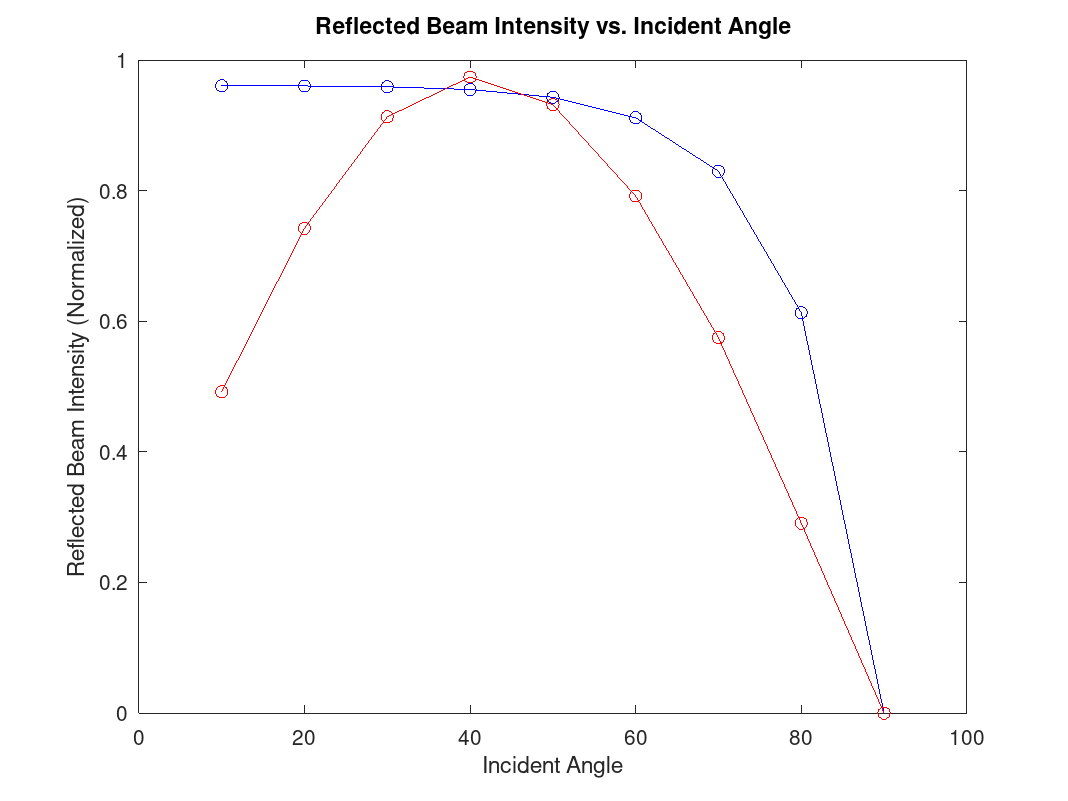
\includegraphics[width=.9\textwidth]{Figures/Lab Seven/Lab7Plot.png}
  \label{fig:1}
\end{figure}

\section{Conclusion}

\subsection{Questions}

\begin{enumerate}

  \item  Calculate the Reflected beam intensity vs incident angle using the equations for TE and TM mode and plot them using software such as MATLAB and Mathematica. The reflective index should be set as the value you got for plexiglass

    Refer to Figure \ref{fig:1} above.

  \item Repeat plot using the experiment results. The beam intensity can be calculated from the measured voltages, normalized to their maximum value.

    Refer to Figure \ref{fig:1} above.


  \item Evaluate the Brewster angle. Are they in line with your expectations? Why?

    We can see from Figure \ref{fig:1}, the point at which reflection is zero is $\theta_i=90^{\circ}$. This makes sense logically, as the light passing through the polarizing filter would be unaffected at an angle of $90^{\circ}$, which would allow the maximum amount of power to be transmitted.

  \item Add loss to the refractive index and calculate it again, describe your observation.

    By adding loss (using the index of refraction obtained in the previous lab), we get the following theoretical graph:

\begin{figure}[H]
  \centering
  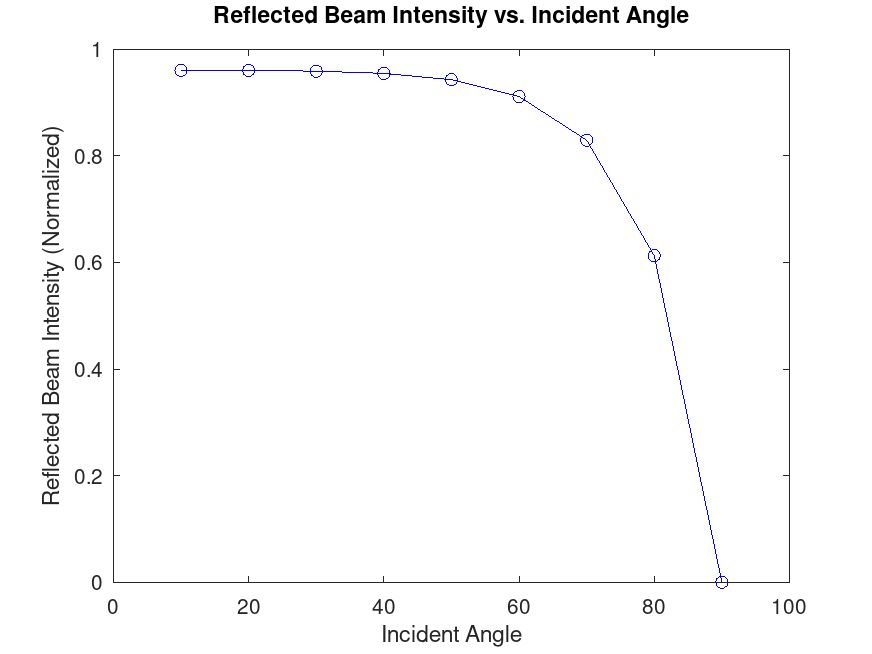
\includegraphics[width=.9\textwidth]{Figures/Lab Seven/Lab7Plot2.png}
  \label{fig:2}
\end{figure}

We can see that the Brewster angle is the same, despite the added loss.

\end{enumerate}

\subsection{Summary}

Overall, through this laboratory experiment, we were able to successfully determine the Brewster angle of the polarizing glass. We did this by measuring the power transmitted and finding the angle of incidence at which this was a maximum (or the reflection was minimized).

\end{document}
